\documentclass[11pt]{article}

\usepackage{amsmath,amsfonts,amssymb,amsthm}
\usepackage[margin=1in]{geometry}
\usepackage[colorlinks]{hyperref}
\usepackage{enumitem}
\usepackage{xcolor}
\usepackage{caption}
\usepackage{graphicx}

\newcommand{\C}{{\mathbb{C}}}
\newcommand{\F}{{\mathbb{F}}}
\newcommand{\R}{{\mathbb{R}}}
\newcommand{\Z}{{\mathbb{Z}}}
\newcommand{\norm}[1]{\|{#1}\|}
\newcommand{\Norm}[1]{\left\|{#1}\right\|}

\newcommand{\red}[1]{{\color{red}#1}}

\newcommand{\eq}[1]{(\ref{eq:#1})}
\renewcommand{\sec}[1]{Section~\ref{sec:#1}}

\begin{document}

%%%%%%%%%%%%%%%%%%%%%%%%%%%%%%%%%%%%%%%%%%%%%%%%%%%%%%%%%%%%%%%%%%%%%%%%%%%%%%

\title{Using Information Entropy to Measure the Merits of Contract Bridge Bidding Systems}

\author{Fanghao Shao 521070910035}

\date{2023-5-23}
\maketitle

\begin{abstract}
A few sentences here: the background of the topic, and what this paper covers.
\end{abstract}

%%%%%%%%%%%%%%%%%%%%%%%%%%%%%%%%%%%%%%%%%%%%%%%%%%%%%%%%%%%%%%%%%%%%%%%%%%%%%%

\section{Introduction}\label{sec:intro}
\paragraph{Motivations.}
% 桥牌是一项多人智力竞技运动,因其简单的规则和激烈的竞争而广受喜爱。桥牌叫牌过程是其非常重要的一环,一个好的叫牌过程往往能清楚地向同伴传递信息,并确定最佳定约。不同的叫牌体系之间各个叫品表达的意义有所不同,使用不同叫牌体系可能导致的最终结果也有所出入,现阶段成熟的叫牌体系主要有自然、精确等,各个体系之间总体较难区分孰优孰劣,但我们可以在每一个单独的叫品上研究每个叫品所传达的具体信息,由此来判断叫牌过程的合理性。//
Contract Bridge (Bridge for short below) is a popular intellectual sport that involves multiple players, simple rules and intense competition. The bidding process is a very important part of bridge, as a good bidding process can convey information clearly to the partner and determine the best contract. Different bidding systems have different meanings for each bid, and using different bidding systems may lead to different final results. At present, mature bidding systems include natural, precision and others, and it is generally difficult to distinguish which system is better or worse. However, we can study the specific information conveyed by each bid and judge the rationality of the bidding process accordingly.

\paragraph{Main results.}
% Give the basic definitions and then the main results that you would like to introduce. Could be helpful to have one or more of the following: a theorem; a table; a figure.
% 本文主要研究同队牌手在寻求最佳定约时叫品所传达的信息,桥牌的叫牌过程可以看作一个带噪声的随机过程,我们需要根据噪声还原内容来确定传递的信息。即便不同的叫牌体系有差距,但是叫品的作用大致可分为几类:自然叫品、限制性叫品、强制性叫品、无限制性叫品和约定叫品。限制性叫品传递的信息量较多,信息熵较小,自然叫品的传递的信息量较少,信息熵较大。适当增加约定叫品虽然会牺牲一些自然叫品能覆盖的含义,但是在有限的叫牌空间下能更加有效地传递同伴所需要的信息,由此来达成合适的定约。//
This paper mainly studies the information conveyed by the bids of the same team players when seeking the best contract, the bidding process in Bridge can be regarded as a noisy random process, and we need to determine the information transmitted based on the noise reduction. Even though different bidding systems have gaps, the functions of the bids can be roughly divided into several categories: natural bids, limiting bids, forcing bids, unlimited bids and conventional bids. Limiting bids convey more information and have smaller information entropy, while natural bids convey less information and have larger information entropy. Adding conventional bids appropriately may sacrifice some meanings covered by natural bids, but it can convey the information needed by the partner more effectively in the limited bidding space, and thus reach a suitable contract.

% \paragraph{Organization.}
% The result of the paper is organized as follows. In Section ..., we .... xxx is presented in Section xxx. Finally, we conclude in Section ....

%%%%%%%%%%%%%%%%%%%%%%%%%%%%%%%%%%%%%%%%%%%%%%%%%%%%%%%%%%%%%%%%%%%%%%%%%%%%%%

\section{Preliminaries}\label{sec:prelim}
% Introduce necessary background knowledge here. 
% 桥牌的基本叫品由定约数与定约花色组成,定约数从1至7代表所需赢的墩数,定约花色之间的大小从高到低依次为无将(NT)、黑桃(S)、红桃(H)、方块(D)、草花(C),以及不叫、加倍和再加倍这三种叫品。叫牌过程中基本叫品只能逐级递增,加倍只能用于对方争叫基本叫品后,再加倍只能用于对方加倍后。本文处于简化目的不考虑防守方的争叫。//定约的最终结果决定分数,真实的情况更为复杂,但我们只考虑如下简单情况。当打牌过程结束后,完成部分定约则奖励50分,完成成局定约奖励300分,完成小满贯定约奖励500分,完成大满贯定约奖励800分,其中最终叫品为3NT及以上,4S、4H及以上,5D、5C及以上为成局定约,任何6阶定约为小满贯定约,任何7阶定约为大满贯定约。因此,桥牌的叫牌过程中应尽量避免将可能成局或满贯的牌停在了低阶定约上,这将造成巨大的损失。
The basic bids in bridge consist of a level and a suit, where the level from 1 to 7 indicates the number of tricks needed to win, and the suits in descending order are no trump (NT), spades (S), hearts (H), diamonds (D), clubs (C), as well as three other bids: pass, double and redouble. The bidding process follows the rule of increasing bids, where double can only be used after the opponents bid a basic bid, and redouble can only be used after the opponents double. For simplification purposes, this paper does not consider the interference bids from the defenders.

The final result of the contract determines the score, it is more complex to simulate a real Bridge bidding and scoring, so we just consider more simple condition. When the play is over, completing a partial contract awards 50 points, completing a game contract awards 300 points, completing a small slam contract awards 500 points, and completing a grand slam contract awards 800 points. The game contracts are any bid of 3NT or higher, 4S or 4H or higher, 5D or 5C or higher. Any bid of level 6 is a small slam contract, and any bid of level 7 is a grand slam contract. Therefore, the bidding process in bridge should avoid stopping at a low-level contract when a game or slam contract is possible, as this would result in a huge loss.

%%%%%%%%%%%%%%%%%%%%%%%%%%%%%%%%%%%%%%%%%%%%%%%%%%%%%%%%%%%%%%%%%%%%%%%%%%%%%%

\section{The bidding logistics}
% 我们以自然叫牌体系为例,叫牌基本原则是,在同伴传递点力信息后计算最低点力达到进局要求时采用非限制性叫品或强制性叫品来逼叫,在点力不确定能否稳定进局时采用限制性叫品或自然叫品邀请进局,在点力明确达不到进局实力时采用限制性叫品示弱结束叫牌。在确定将牌花色上主要寻求高花配合,牺牲了少部分低花叫品为约定叫品和强制性叫品,在高花失配时选择无将定约。
We take the natural bidding system as an example. The basic principle of bidding is to use non-limiting bids or forcing bids to  force the bidding after the partner conveys the point count information, to use limiting bids or natural bids to invite the game when the point count is uncertain whether it can reach the game level, and to use limiting bids to show weakness and end the bidding when the point count is clearly not enough for the game. In determining the trump suit, the main goal is to seek high suit fit, sacrificing some low suit bids for conventional bids and forcing bids. When the high suits are mismatched, choose no trump contract.

% 例如你的同伴开叫 1S ,代表你11个hpc以上,21个hpc以下,5张以上黑桃。你手持4张黑桃,但只有4个hpc,你应该选择 3S 代表我的手牌中有4张以上黑桃,但是只有5个hpc以下,我没有其他更多实力了。当你的同伴有18个hpc以上并且有很好的控制(比如其他花色单缺)时才有信心加叫到 4S 进局,否则你的同伴就知道了你的牌上限而选择 Pass 停止叫牌。
For example, your partner opens 1S, which means he has 11 or more high card points(hcp) and 21 or less hcp, and 5 or more spades. You have 4 spades, but only 4 hcp. You should choose 3S to indicate that you have 4 or more spades in your hand, but only 5 or less hcp,and have no more strength. Only when your partner has 18 or more hcp and good control (such as a singleton in another suit) can he be confident to bid 4S to reach the game. Otherwise, your partner knows your upper limit and chooses Pass to stop the bidding.

% 在这里,你的 3S 就是限制性叫品。它明确表达了自己的点力上限,传递的信息量大而信息熵小。同时你和同伴至少 5-4 配合的黑桃套在大多数情况下能保证定约的完成,即便你的同伴大牌点不足以支撑你完成这个部分定约,也能成功阻击住对手更多牌点的争叫而破坏了他们的局。综合考虑下来,这个叫品的好处是非常明显的。
Here, your 3S is a limiting bid. It clearly expresses your upper limit of points, conveying a large amount of information and having a small information entropy. At the same time, your at least 5-4 fit in spades with your partner can guarantee the completion of the contract in most cases. Even if your partner does not have enough points to support this partial contract, you can also successfully block the opponents’ more points bidding and ruin their game. Considering all these factors, the benefits of this bid are very obvious.

% 我们再考虑另一种情况,你的同伴仍然是以 1S 开叫,但你此时的手牌中有3张黑桃,且有9个hpc。根据你的hpc进行估算,你发现只要你的队友不是开叫实力的最低限(14点以下),那么你们就很有希望做成 4S 成局定约,此时你应该选择 2S 平加叫。这里的 2S 是自然叫品,它虽然界定了你的调整点(根据将牌黑桃以及你的牌型对你的大牌点实力进行调整后的点力)范围为7到10,但是它并没有说明任何其他的信息,也就是信息熵较大,你让同伴来判断是否能够完成成局定约。
Let’s consider another situation. Your partner still opens 1S, but this time you have 3 spades and 9 hcp in your hand. Based on your high card points estimation, you find that as long as your partner is not at the lowest limit of opening strength (below 14 points), then you have a good chance of making a 4S game contract. In this case, you should choose 2S to raise. Here, 2S is a natural bid. It defines your adjustment point (according to your trump suit-spades and your hand shape, you may adjust your point) range as 7 to 10, but it does not specify any other information, that is, it has a large information entropy. You let your partner judge whether he can complete the game contract.

% 那么我们能否将这两种叫品的含义反过来呢?当然可以!并且这种用法也是存在的,但效果并不好。因为叫品的阶数越高,留下的叫牌空间就越小,倘若你到此刻还没能表达清楚自己的牌力范围,自己能否成局,停留在一个较大的信息熵中,那么这个叫品必然是失败的。
However we can reverse the meanings of the two bids, but this usage does exist, but it is not effective. Because the higher the level of the bid, the smaller the bidding space left. If you have not been able to express your point range clearly, whether you can reach the game, and stay in a larger information entropy, then this bid is bound to be a failure.

% 如何保证在叫牌阶数增加的同时降低信息熵,尽可能地表达出自己的牌情以便同伴判断,自然叫牌体系有两种手段:一是将更多的叫牌空间留给无限制性叫品、强制性叫品和自然叫品,二是将部分自然叫品转化为约定叫品。在上面的例子当中,我们就展示了第一种手段的好处:将 3S 设置为限制性叫品,2S 为自然叫品。这个做法乍一看令人费解,但继 2S 之后的可选择空间比 3S 多了4种,也使得双方有更多的能力探求边花上的配合。例如开叫者回叫 3D 就表示自己有3张以上的方块套,邀请你在方块套较长或有好控制时进局,即便你和同伴在方块上不搭也能重新回到 3S,保证定约不会被打宕。第二种手段类似于分割了自然叫品的一些叫牌情况,在牺牲掉一些几乎无用的自然叫品后来代表一些其他情况,能更清楚地传递信息。下面我们再来看一个例子。
How to ensure that the information entropy is reduced while the bidding level is increased, and express one’s own hand situation as much as possible for the partner to judge. The natural bidding system has two means: one is to leave more bidding space for unlimited bids, forcing bids and natural bids, and the other is to transform some natural bids into conventional bids. In the above example, we showed the benefits of the first method: setting 3S as a limiting bid and 2S as a natural bid. This approach seems puzzling at first glance, but after 2S, there are four more options than after 3S, which also gives both sides more ability to explore the fit in the side suits. For example, if the opener bids 3D, it indicates that he has 3 or more diamonds and invites you to bid game if you have a long or good control in diamonds. Even if you and your partner do not fit in diamonds, you can return to 3S and ensure that the contract will not be defeated. The second method is similar to splitting some situations of natural bids, and conventionally using some other bidding, which can convey information more clearly. Here's an another example.

% 同样还是你的同伴开叫 1S,此时你和你的同伴有约定叫品:3C、3D,他们分别代表了你的牌点在7-9、10-12,同时二者均保证了黑桃有4张支持。在你们没有约定之前,3C、3D所代表的意义分别是草花、方块的弱单套阻击叫,假如你有4张黑桃支持你应该根据你的点力范围选择叫 2S、3S。可以发现,在约定这个叫品之前,2S、3S的含义太广了,使得同伴无法判断你们真实的能力范围,并且弱单套阻击的意义在你队友开叫保证11个hpc之后意义不大,出现的频率也不高。因此,舍弃这两种低频且收益低的叫品来代表更为精确的叫品,能为叫牌带来不少优势。
The same as before, your partner opens 1S. This time you and your partner have a conventional bid: 3C and 3D. They respectively indicate that your hcp is 7-9 and 10-12, and both guarantee 4 spades support. Before you agreed on this bid, the meanings of 3C and 3D were weak but long in clubs or diamonds for preemptive bids. You should choose to bid 2S or 3S according to your point range if you have spades support instead. You can see that before agreeing on this bid, the meanings of 2S and 3S were too broad, making it difficult for your partner to judge your true ability range. And the meaning of weak singletons for preemption is not very significant after your partner opens with 11 hpc guaranteed, and the frequency of occurrence is not high either. Therefore, giving up these two low-frequency and low-benefit bids to represent more precise bids can bring a lot of advantages to the bidding.
%%%%%%%%%%%%%%%%%%%%%%%%%%%%%%%%%%%%%%%%%%%%%%%%%%%%%%%%%%%%%%%%%%%%%%%%%%%%%%

\section{Methods}
% May also have only one technical section, depending on the materials you cover.
% 为了衡量叫品所传达的信息,我们选取了一个特定的叫牌过程,构造可能出现的牌例,编写简单叫牌逻辑分别测试了使用不同叫品体系的最终结果,并使用双明手结果(Double Dummy Solver)分析牌例最终能够完成的定约进行比较,一个好的叫品应该能让最终叫品与双明手结果一致,同时根据可能出现的牌例比例测算信息熵。最终结果如下:
To measure the information conveyed by the bids, we selected a specific bidding process(opens 1S and ends with Spades), constructed possible hands, wrote simple bidding logic to test the final results using different bidding systems, and used double dummy solver to analyze the final contract that could be completed by the hands for comparison. A good bid should make the final bid consistent with the double dummy result, and calculate the information entropy based on the proportion of possible hands. The final results are shown at Table 1 and 2 and Figure 1.


\begin{center}
    \begin{tabular}{|l|r|r|r|r|r|}
        \hline
         & Grand Slam & Small Slam & Game & Part Score & Other \\
        \hline
        Total & 1195 & 2778 & 7923 & 4227 & 972 \\
        \hline
        Overbid & - & 103 & 1032 & 1442 & 416 \\
        \hline
        Just Right & 498 & 1468 & 5899 & 2785 & 128 \\
        \hline
        Underbid & 697 & 1207 & 992 & - & 428 \\
        \hline
    \end{tabular}
\end{center}

\captionof{table}{Simple natural bidding simulation}

\begin{center}
    \begin{tabular}{|l|r|r|r|r|r|}
    \hline
     & Grand Slam & Small Slam & Game & Part Score & Other \\
    \hline
    Total & 1195 & 2778 & 7923 & 4227 & 972 \\
    \hline
    Overbid & - & 94 & 1015 & 1034 & 399 \\
    \hline
    Just Right & 567 & 1681 & 6341 & 3193 & 126 \\
    \hline
    Underbid & 628 & 1003 & 567 & - & 447 \\
    \hline
    \end{tabular}
\end{center}
\captionof{table}{Conventional natural bidding simulation}

\begin{figure}
    \centering
    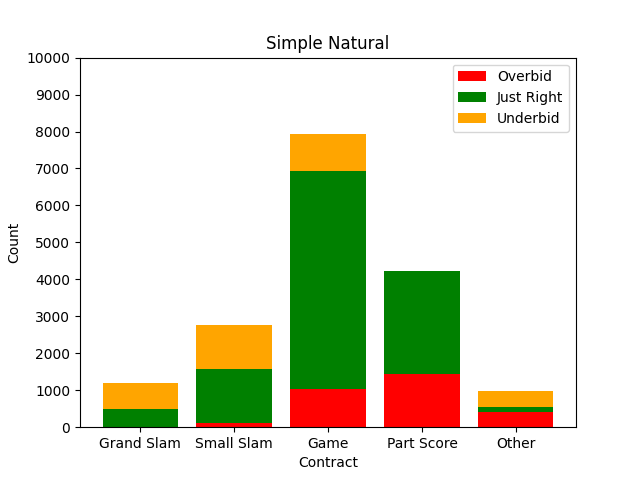
\includegraphics[width=0.4\textwidth]{Figure_1}
    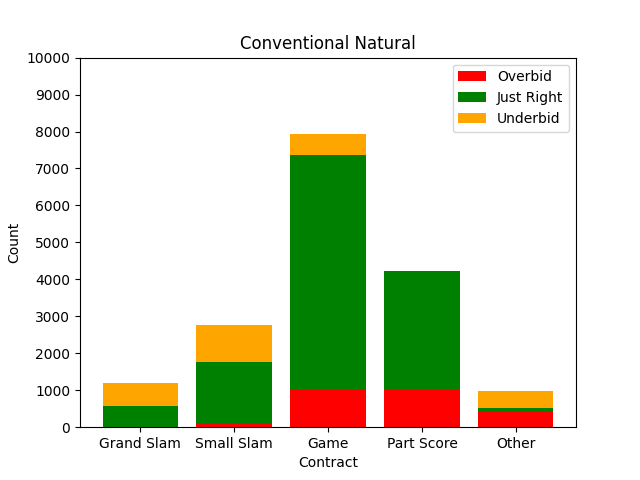
\includegraphics[width=0.4\textwidth]{Figure_2}
    \caption{Comparison of Simple and Conventional natural bidding}
    \label{fig:my_label}
\end{figure}
%%%%%%%%%%%%%%%%%%%%%%%%%%%%%%%%%%%%%%%%%%%%%%%%%%%%%%%%%%%%%%%%%%%%%%%%%%%%%%

\section{Conclusion}
% Potentially two paragraphs: One paragraph summarizing the contents in this paper, and a second paragraph for highlighting future directions and open questions.
% 我所写的叫牌逻辑核心想法是保证不丢失成局定约,并不代表能最正确的结果。根据实验结果可以发现使用部分约定叫后能提升合格率,但是影响较微弱。总的来说使用部分约定叫还是能从一定程度上降低失误率。但从另一角度,过多的约定叫还是会挤压自然叫品和限制性叫品的空间,使得另外可能的配合被忽略。
The core idea of the bidding logic I wrote is to ensure that the game contract is not lost, and it does not mean that it can achieve the most correct result. According to the experimental results, it can be found that using some conventional bids can improve the pass rate, but the effect is weak. Generally speaking, using some conventional bids can reduce the error rate to some extent. As we said before, it worth sacrificing natural bids for a frequent and significant bids which  conveys the information needed by the partner more effectively in the limited bidding space, and thus reach a suitable contract. But from another perspective, too many conventional bids will squeeze the space of natural bids and limiting bids, and ignore other possible fits. 

% 本文并不算是真正意义上的研究,而仅仅是从概率学和信息论的角度还原了一部分叫牌过程,由此来探讨叫牌体系的合理性。未来可以继续研究如何界定约定叫与自然叫等其他叫品之间合理的比例,用数值量化整个过程。
This paper is not a real research, but only restores part of the bidding process from the perspective of probability and information theory, and discusses the rationality of the bidding system. In the future, we can continue to study how to define a reasonable proportion between conventional bids and natural bids and other bids, and quantify the whole process with numerical values.

\section{Appendix}
Source code repository https://github.com/DAntyNoel/Information-Theorem-Bridge
%%%%%%%%%%%%%%%%%%%%%%%%%%%%%%%%%%%%%%%%%%%%%%%%%%%%%%%%%%%%%%%%%%%%%%%%%%%%%%

% \section*{Logistics (Delete this section when you write the final report)}
% \begin{itemize}
% \item Deadline: December 11, 11:59 pm.

% \item The final report should be written by this template and contains at most 10 pages (excluding the references). Scores will be deduced if you do not use this template or write more than 10 pages.

% \item Regarding the content, I expect that introducing and summarizing the key points of the papers you choose will be a main component of the final report. Beyond only summarizing those papers, I expect to further see more comprehensive understanding from your side. For instance, what are the novel contributions they made? What are the open questions that people may work on in the future? Such discussions by yourself are crucial, and go beyond only summarizing existing papers. In all, I would like to see your own understanding of a research topic, both about its content and its further connection.
% \end{itemize}

% The final report counts as 20 points to the final grade. I will evaluate the final report based on the following four perspectives, 5 points for each (see also the slides from the first class):
% \begin{itemize}
% \item Contents: The range and the level of details that the report covers. 

% \item Novelty: Catch the up-to-date trend. 

% \item Clarity: The clarity of the contents, whether those are intuitive and understandable.

% \item Quality: Grammars, choice of words, typos, expression of mathematical formulas, etc.
% \end{itemize}

%%%%%%%%%%%%%%%%%%%%%%%%%%%%%%%%%%%%%%%%%%%%%%%%%%%%%%%%%%%%%%%%%%%%%%%%%%%%%%

\begin{thebibliography}{9}
\bibitem{KT06}
% 李娜. 引入合作竞争关系的桥牌叫牌数据库构建[D]. 北京邮电大学, 2009.
Li Na. Construction of Bridge Bidding Database with Cooperative Competition Relationship[D]. Beijing University of Posts and Telecommunications, 2009.
\end{thebibliography}

\end{document}